% Pdf only
\documentclass[aspectratio=169]{beamer}
% For presentation
%\documentclass[aspectratio=169, notes]{beamer}
\usepackage{lmodern}
\usepackage{pgfpages}
%\setbeameroption{show notes on second screen}
%\usepackage[utf8]{inputenc} 
\usepackage[english]{babel}

%
% Choose how your presentation looks.
%
% For more themes, color themes and font themes, see:
% http://deic.uab.es/~iblanes/beamer_gallery/index_by_theme.html
%
\mode<presentation>
{
  \usetheme[]{metropolis}           % Use metropolis theme
} 

\begin{document}
\obeylines

\title[Open Source SLAM Library for Embedded Systems]{Open Source SLAM Library for Embedded Systems}
\author{Stefan Eichenberger, CPVR Lab}
\date{24.01.2020}

\begin{frame}
  \titlepage\thispagestyle{empty}
\end{frame}

\begin{frame}{Introduction}
  \begin{columns}[c]
    \begin{column}{0.4\linewidth}
      \begin{itemize}
        \item What is SLAM?
        \item What did we do?
        \item Why did we do it?
      \end{itemize}
    \end{column}
    \begin{column}{0.4\linewidth}
      \begin{center}
        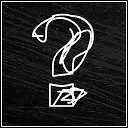
\includegraphics[width=0.5\textwidth]{./img/questionmark.jpg}
      \end{center}
    \end{column}
  \end{columns}
\end{frame}

\begin{frame}{Different SLAMs}
  \begin{center}
    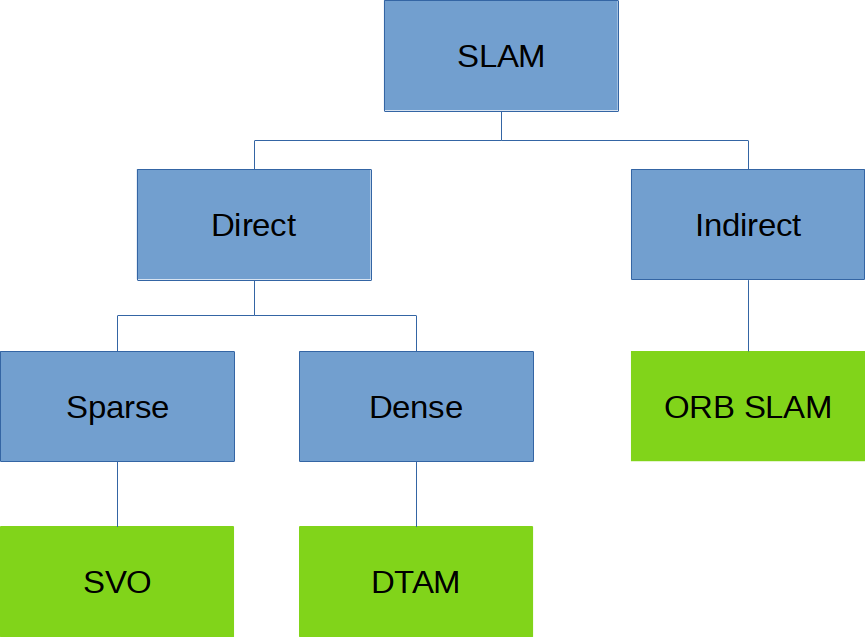
\includegraphics[height=0.9\textheight]{../img/slam_modes.png}
  \end{center}
\end{frame}

\begin{frame}{SVO SLAM}
  \begin{center}
    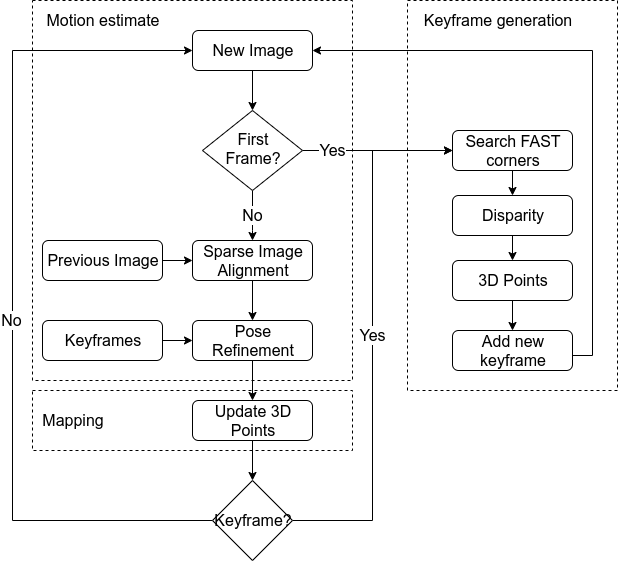
\includegraphics[height=0.9\textheight]{../img/our_svo_slam.png}
  \end{center}
\end{frame}

\begin{frame}{Steps}
  \begin{columns}[c]
    \begin{column}{0.5\linewidth}
      \begin{enumerate}
        \item Maintain 3D point cloud
        \item Pose estimation based on sparse image alignment
        \item Pose refinement based on optical flow
        \item Update 3D point cloud
      \end{enumerate}
    \end{column}
    \begin{column}{0.3\linewidth}
      \begin{center}
        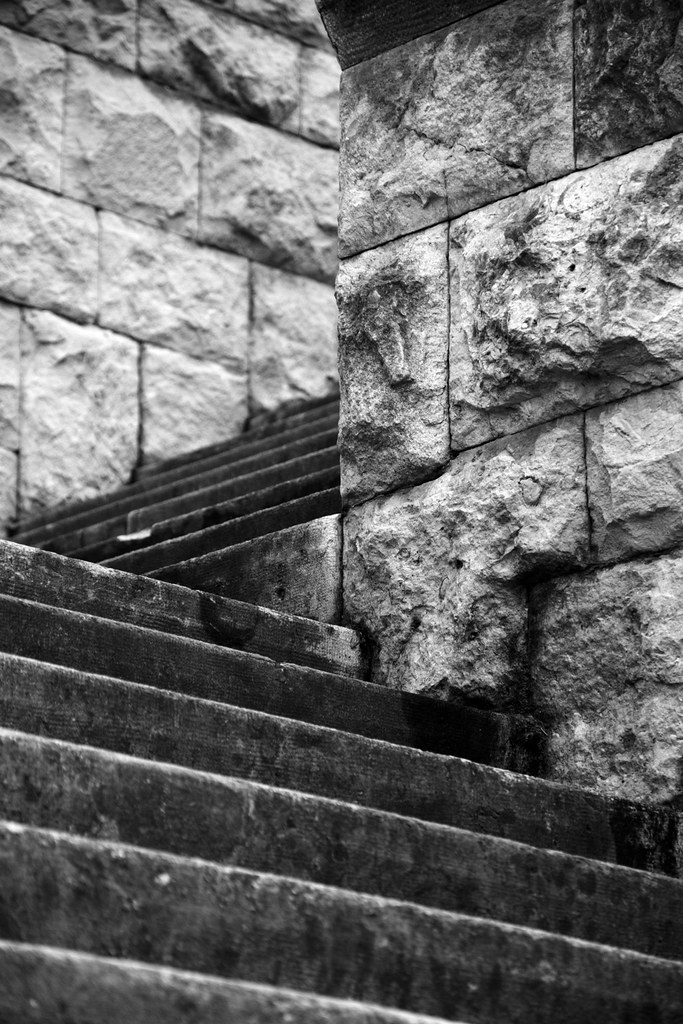
\includegraphics[width=0.8\textwidth]{./img/steps.jpg}
      \end{center}
    \end{column}
  \end{columns}
\end{frame}

\begin{frame}{Maintain 3D Point Cloud (Camera)}
  \begin{center}
    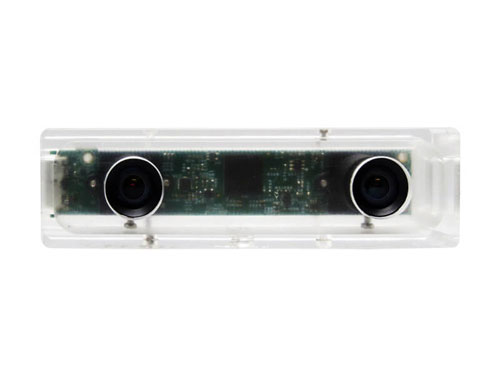
\includegraphics[height=0.9\textheight]{../img/tara_cam.jpg}
  \end{center}
\end{frame}


\begin{frame}{Maintain 3D Point Cloud}
  \begin{center}
    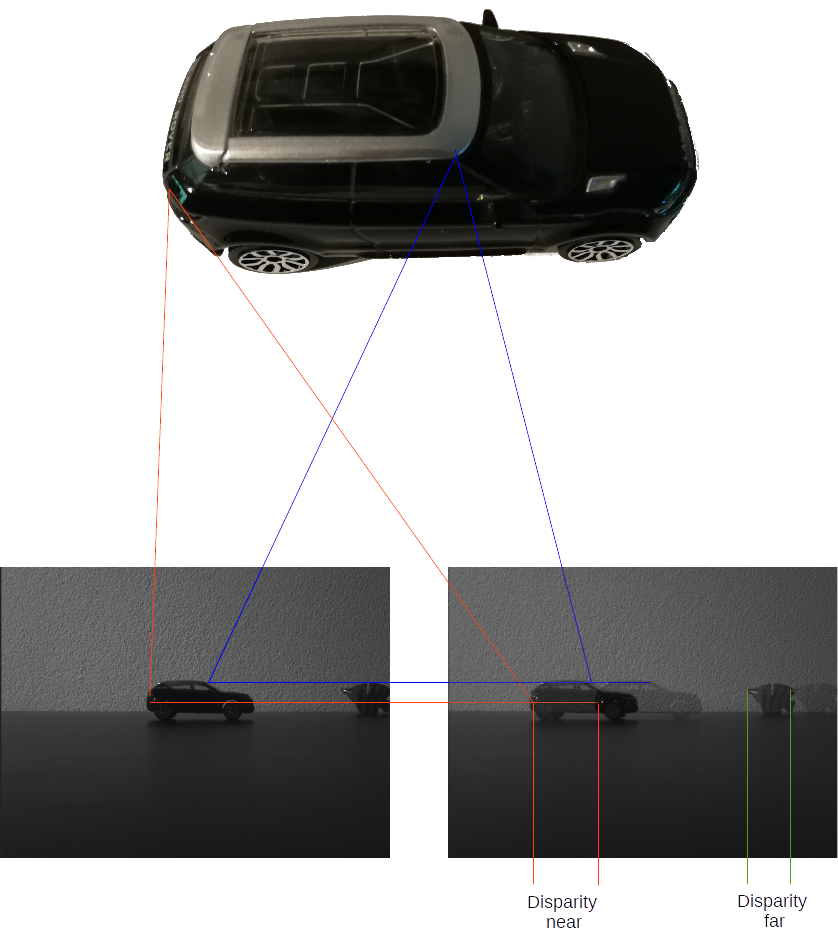
\includegraphics[height=0.9\textheight]{../img/disparity_concept.png}
  \end{center}
\end{frame}

\begin{frame}{Sparse Image Alignment}
  \begin{center}
    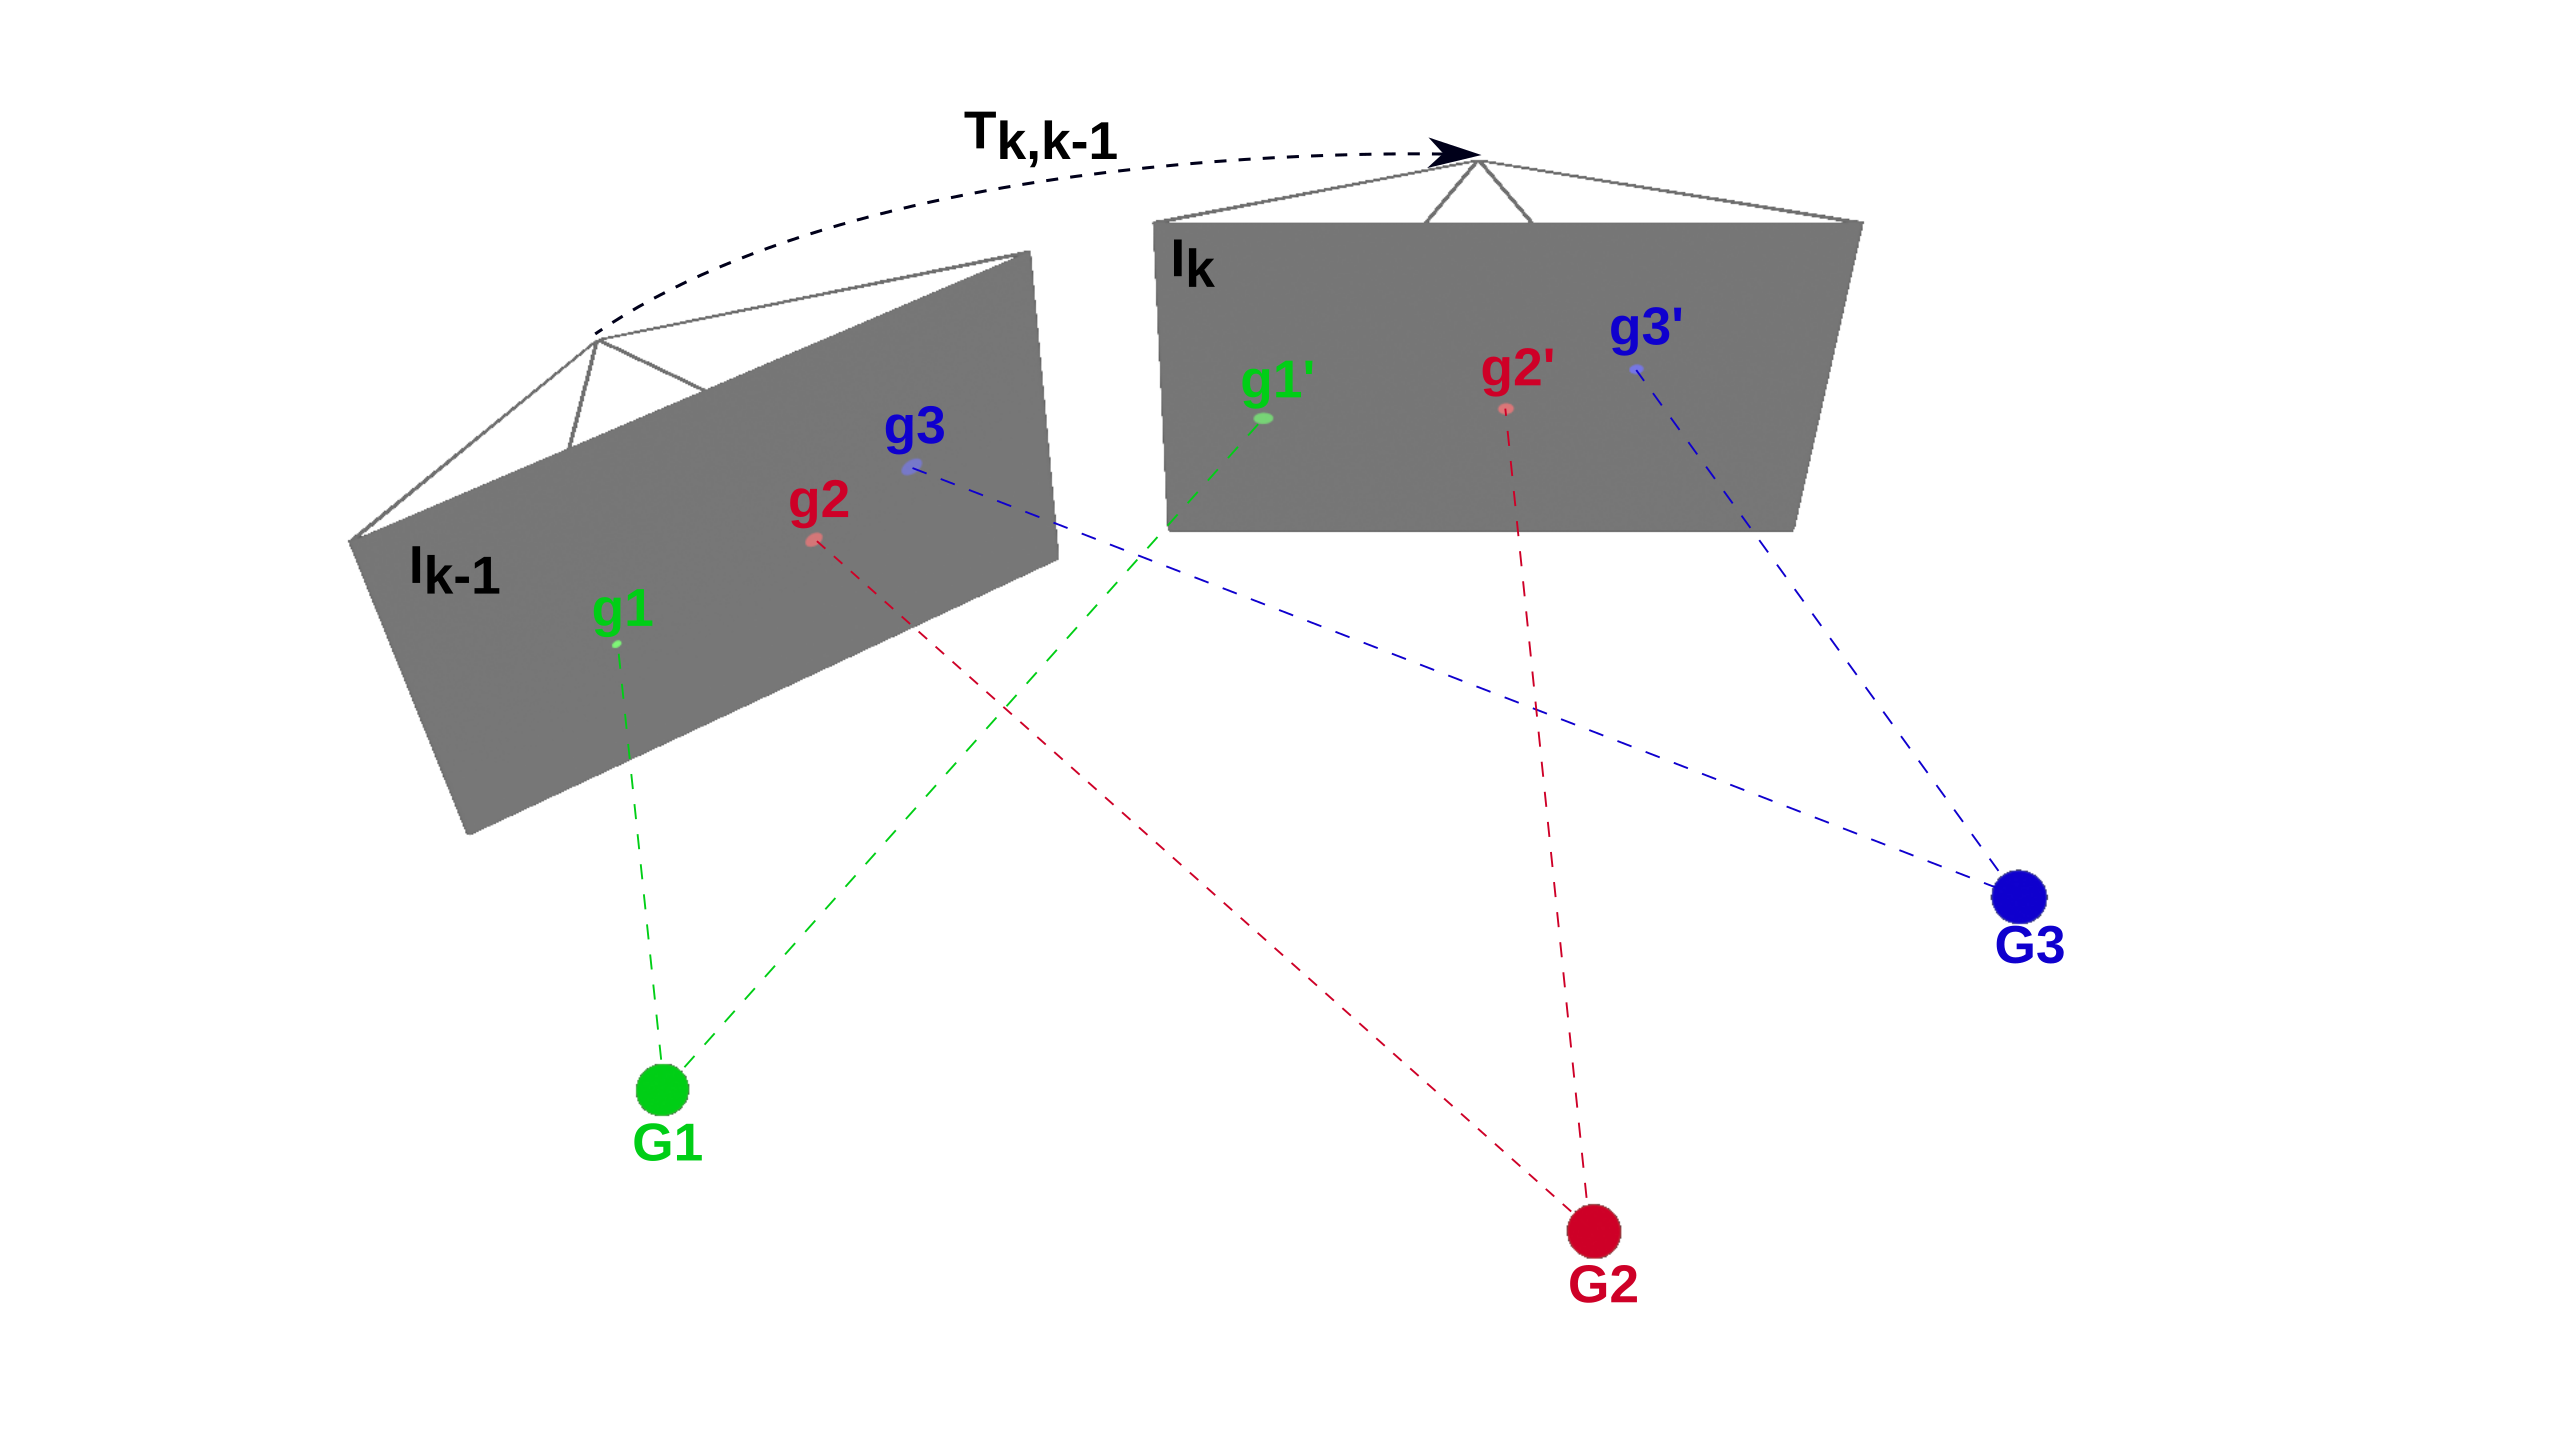
\includegraphics[height=0.9\textheight]{../img/pose_estimation_sparse.png}
  \end{center}
\end{frame}

\begin{frame}{Pose Refinement}
  \begin{center}
    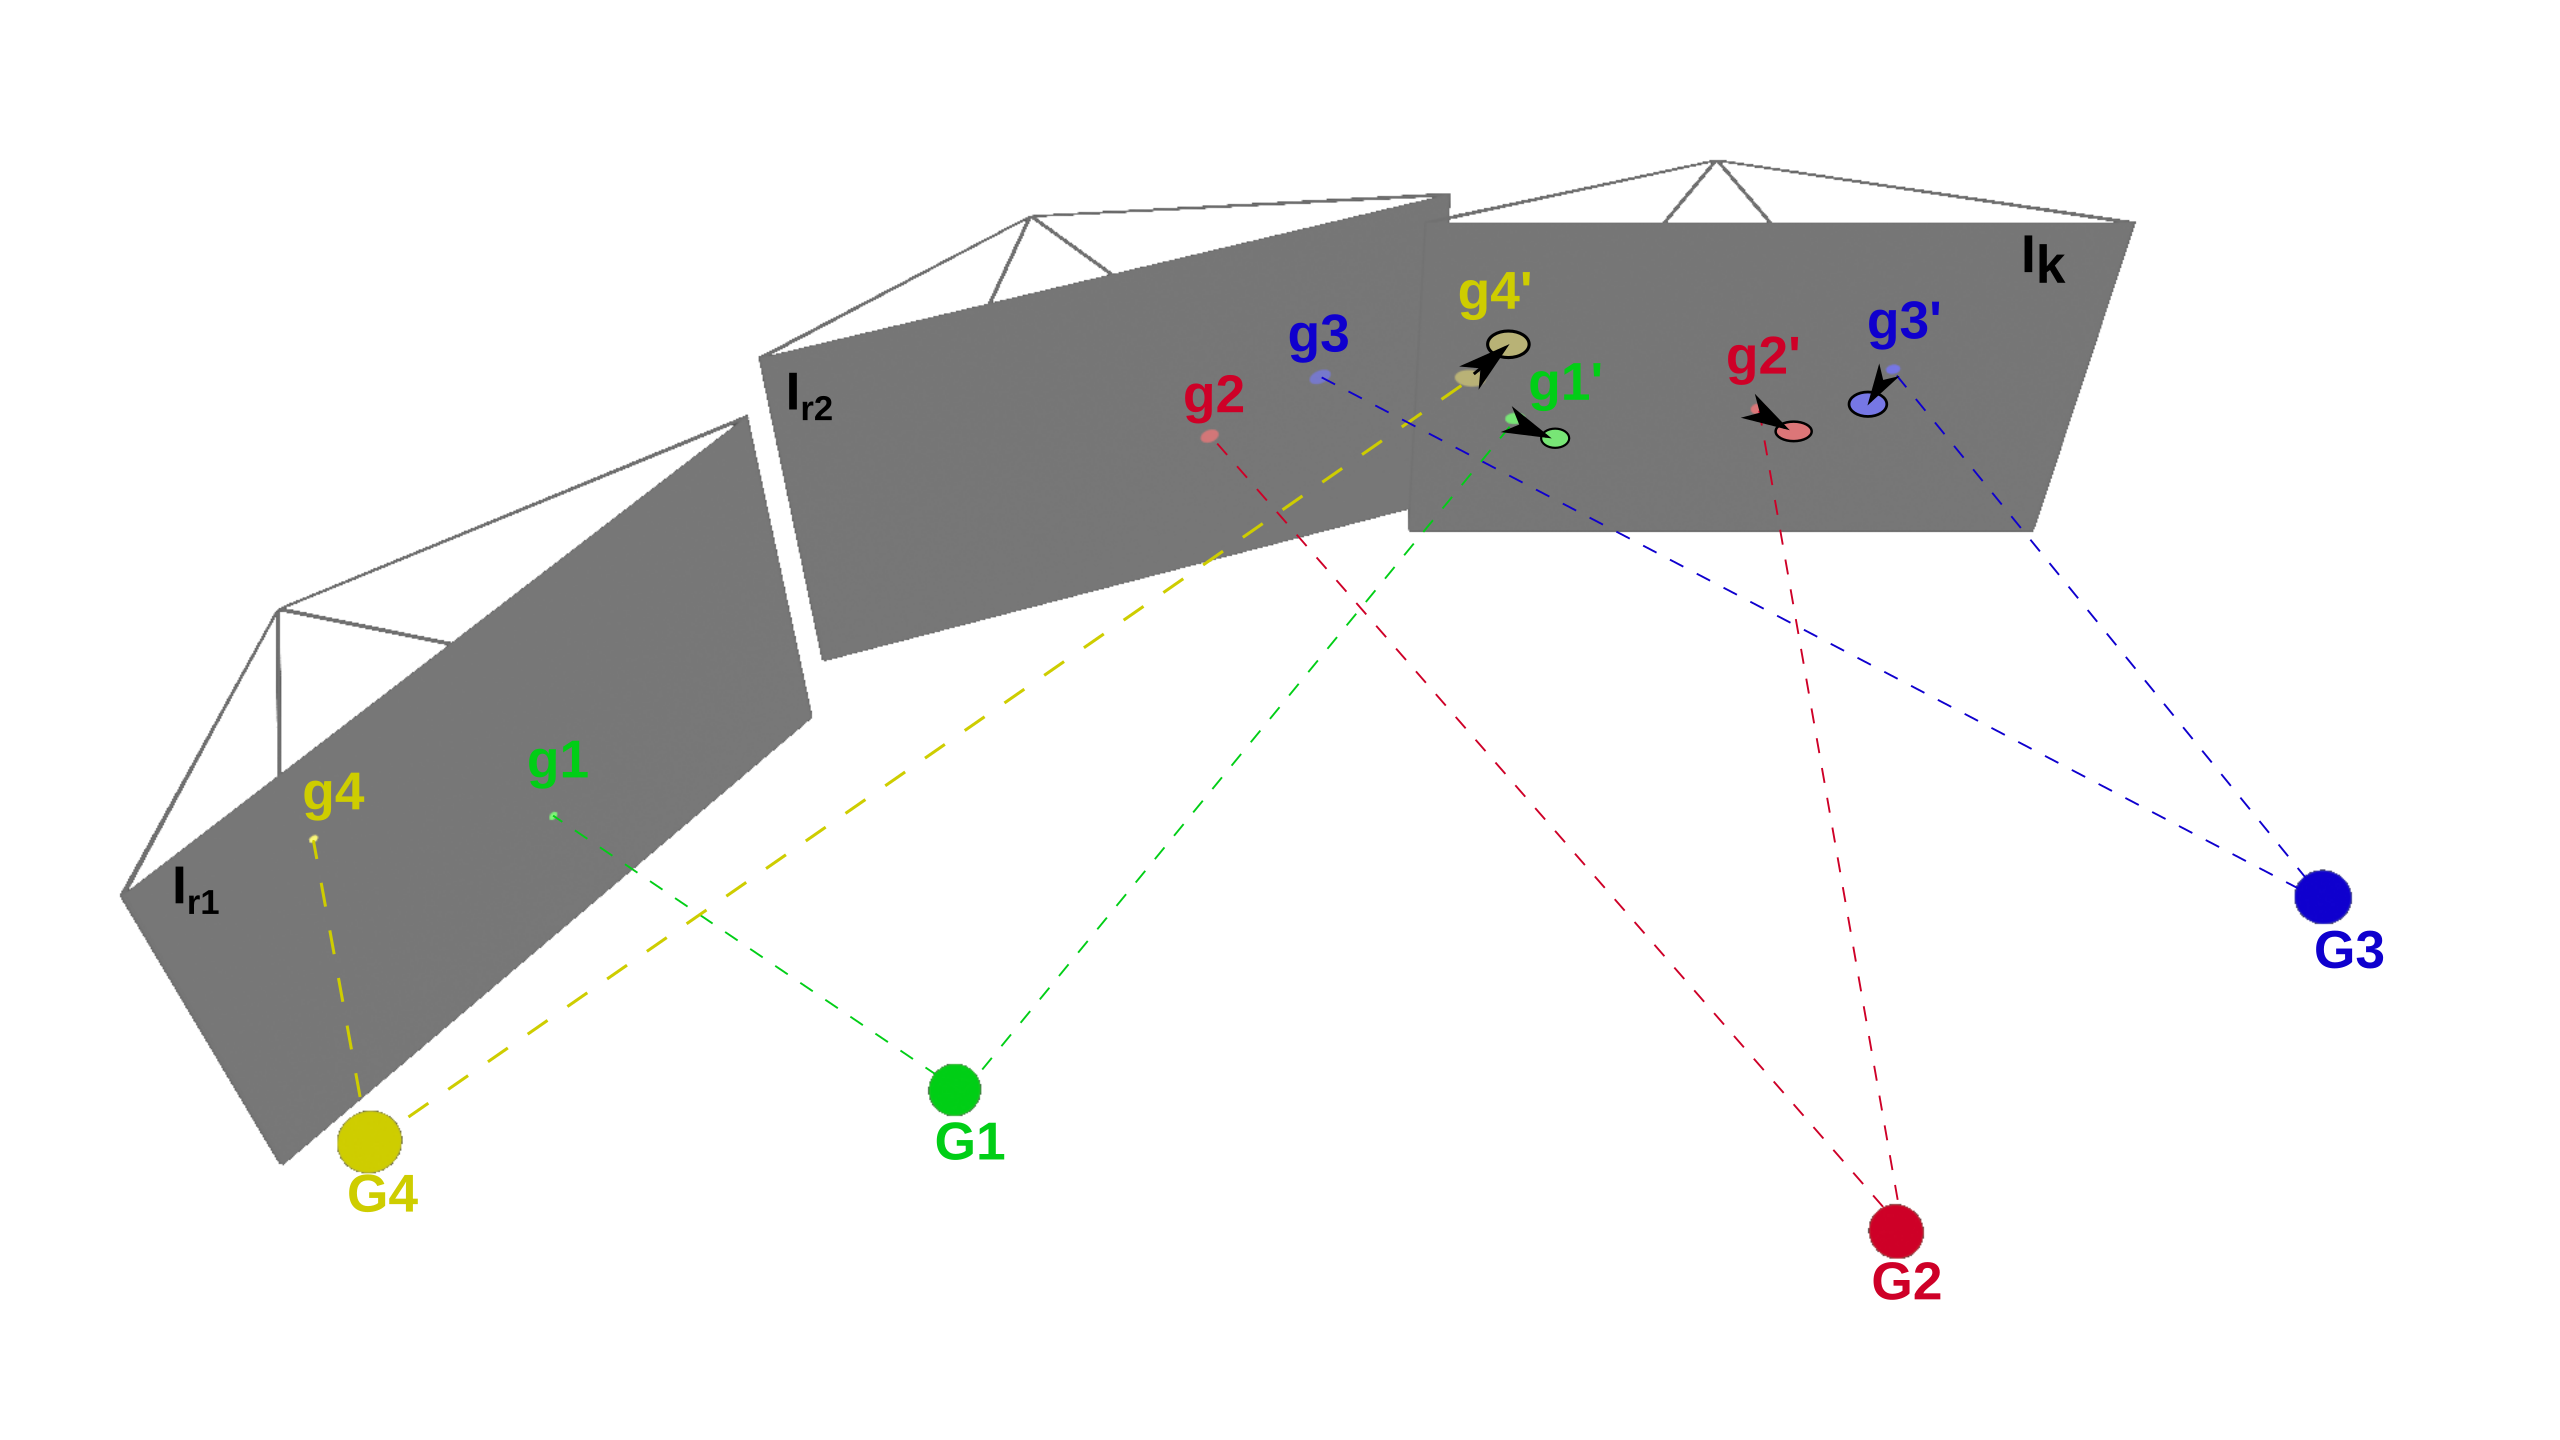
\includegraphics[height=0.9\textheight]{../img/pose_estimation_opt_flow.png}
  \end{center}
\end{frame}

\begin{frame}{Pose Refinement}
  \begin{center}
    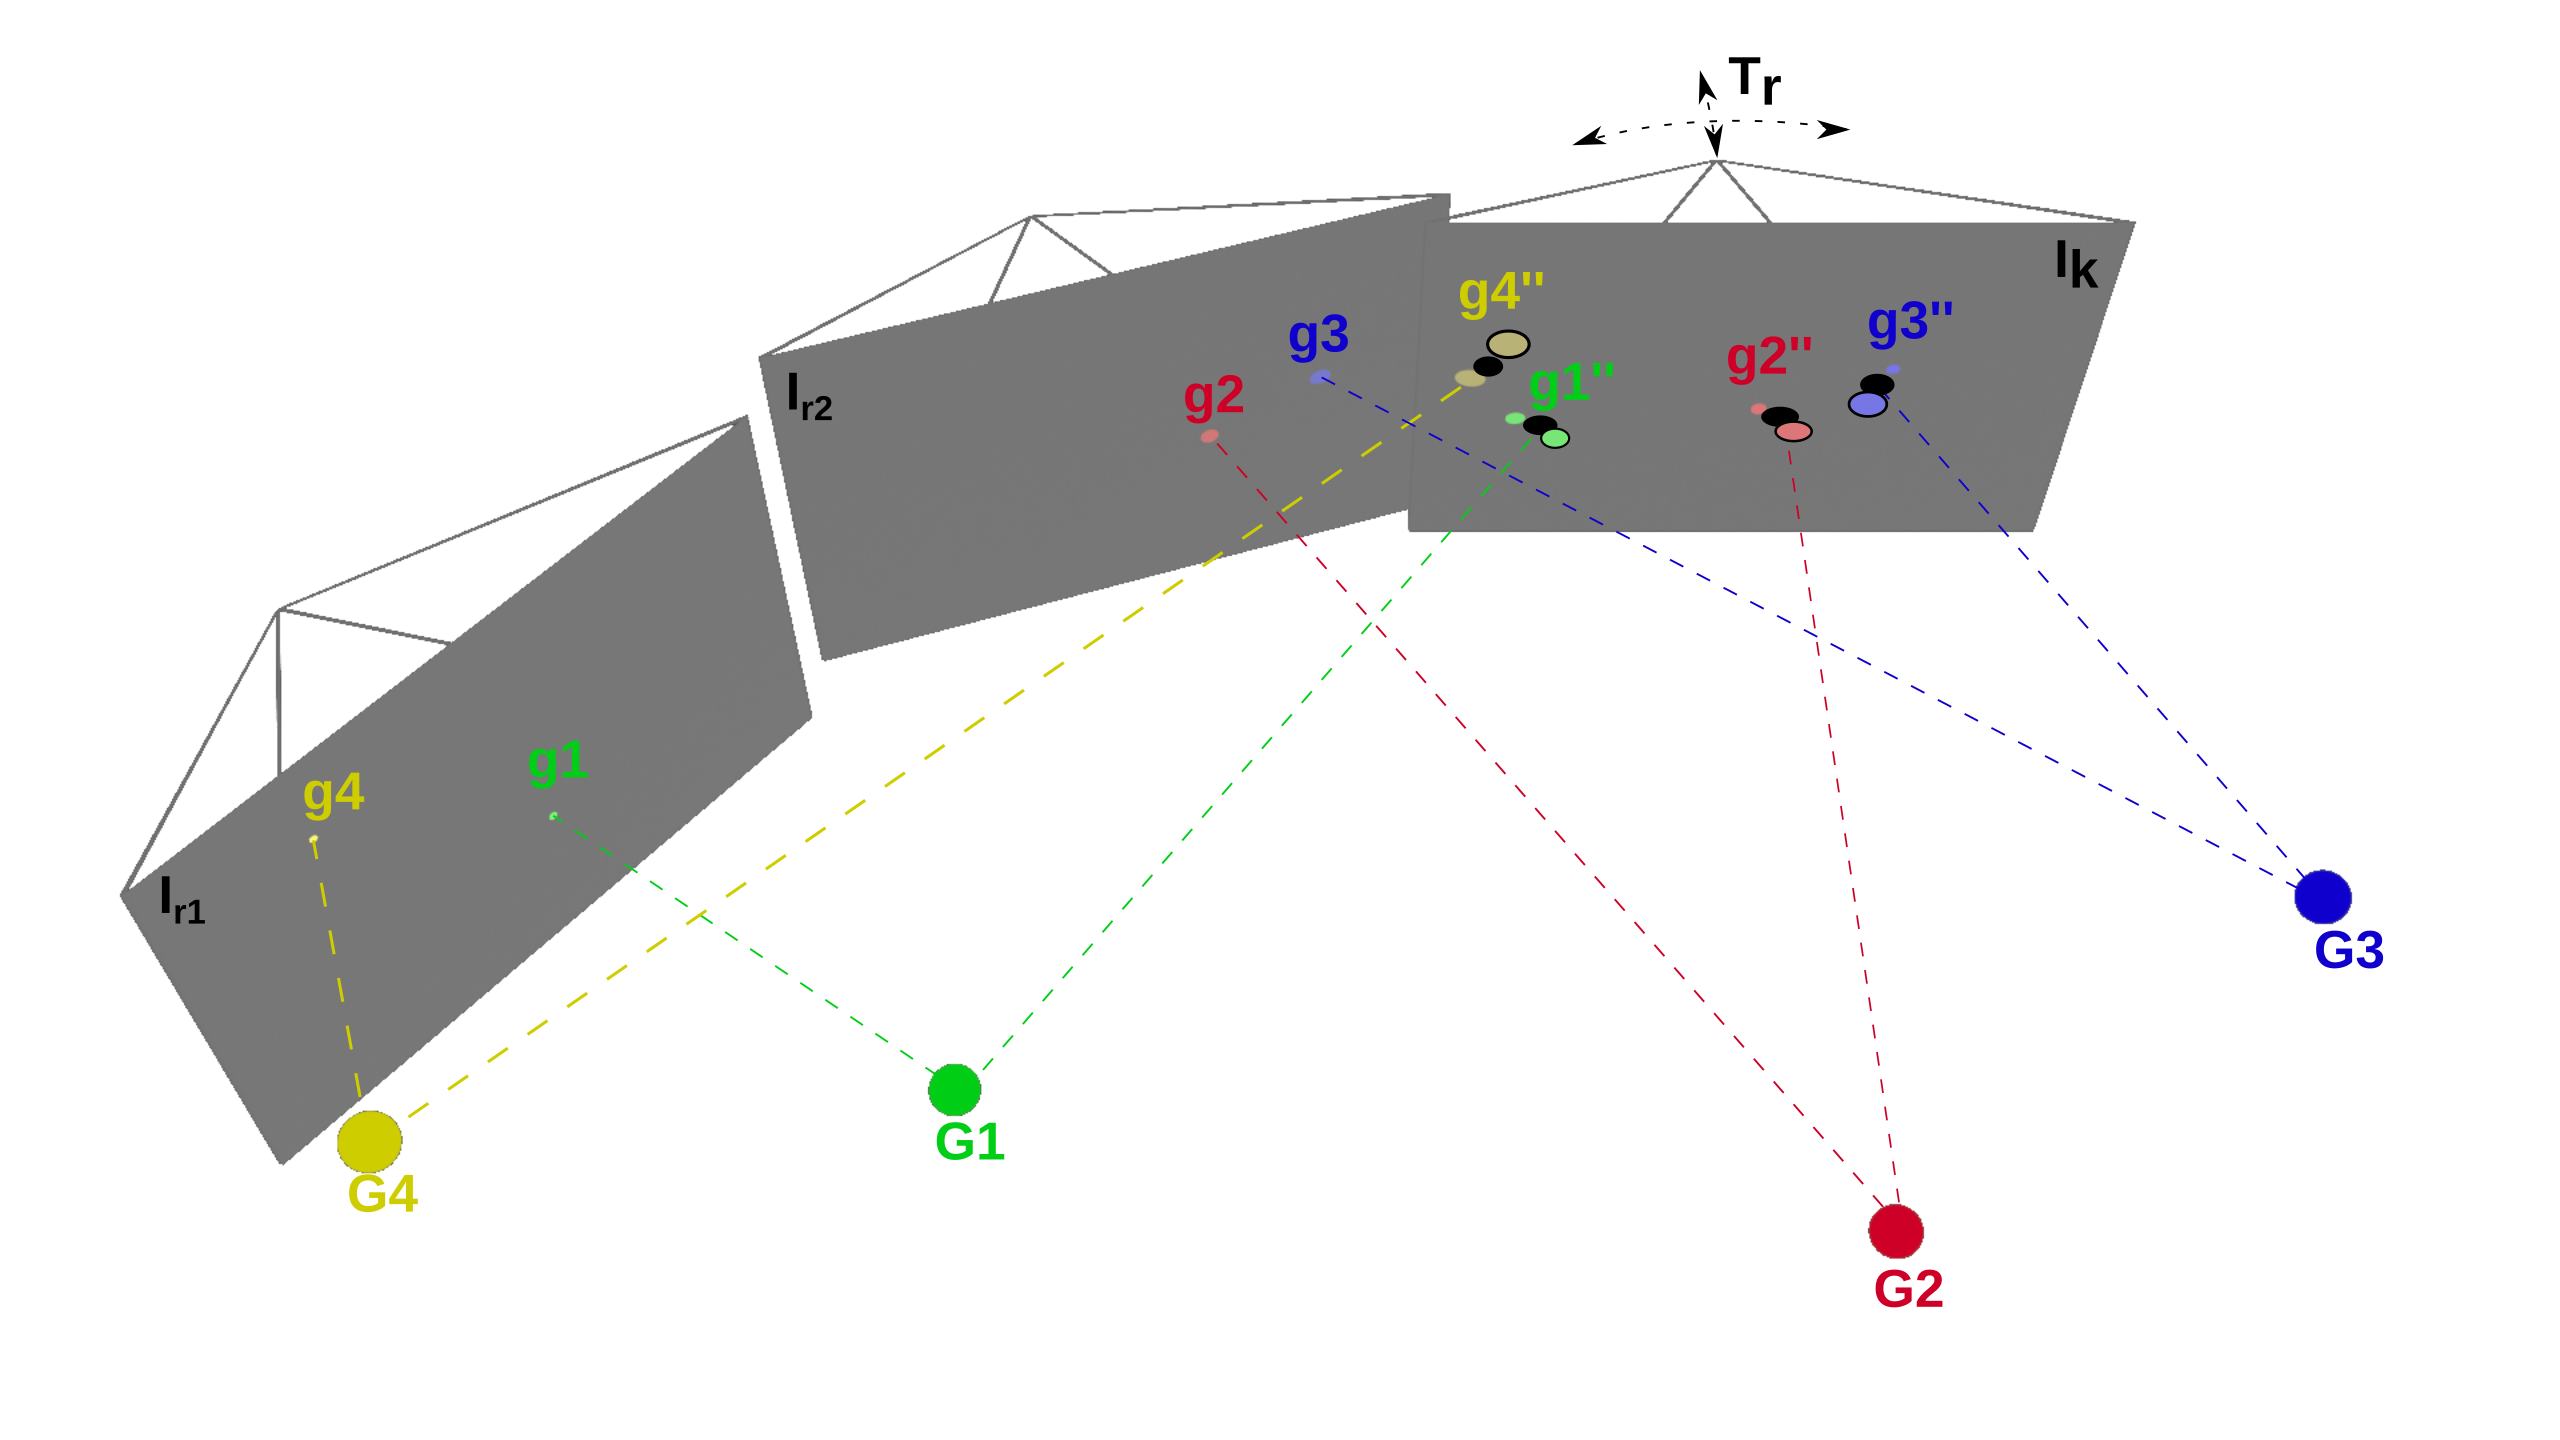
\includegraphics[height=0.9\textheight]{../img/pose_estimation_refinement.png}
  \end{center}
\end{frame}

% TODO!!!
\begin{frame}{3D Point Update}
  \begin{center}
    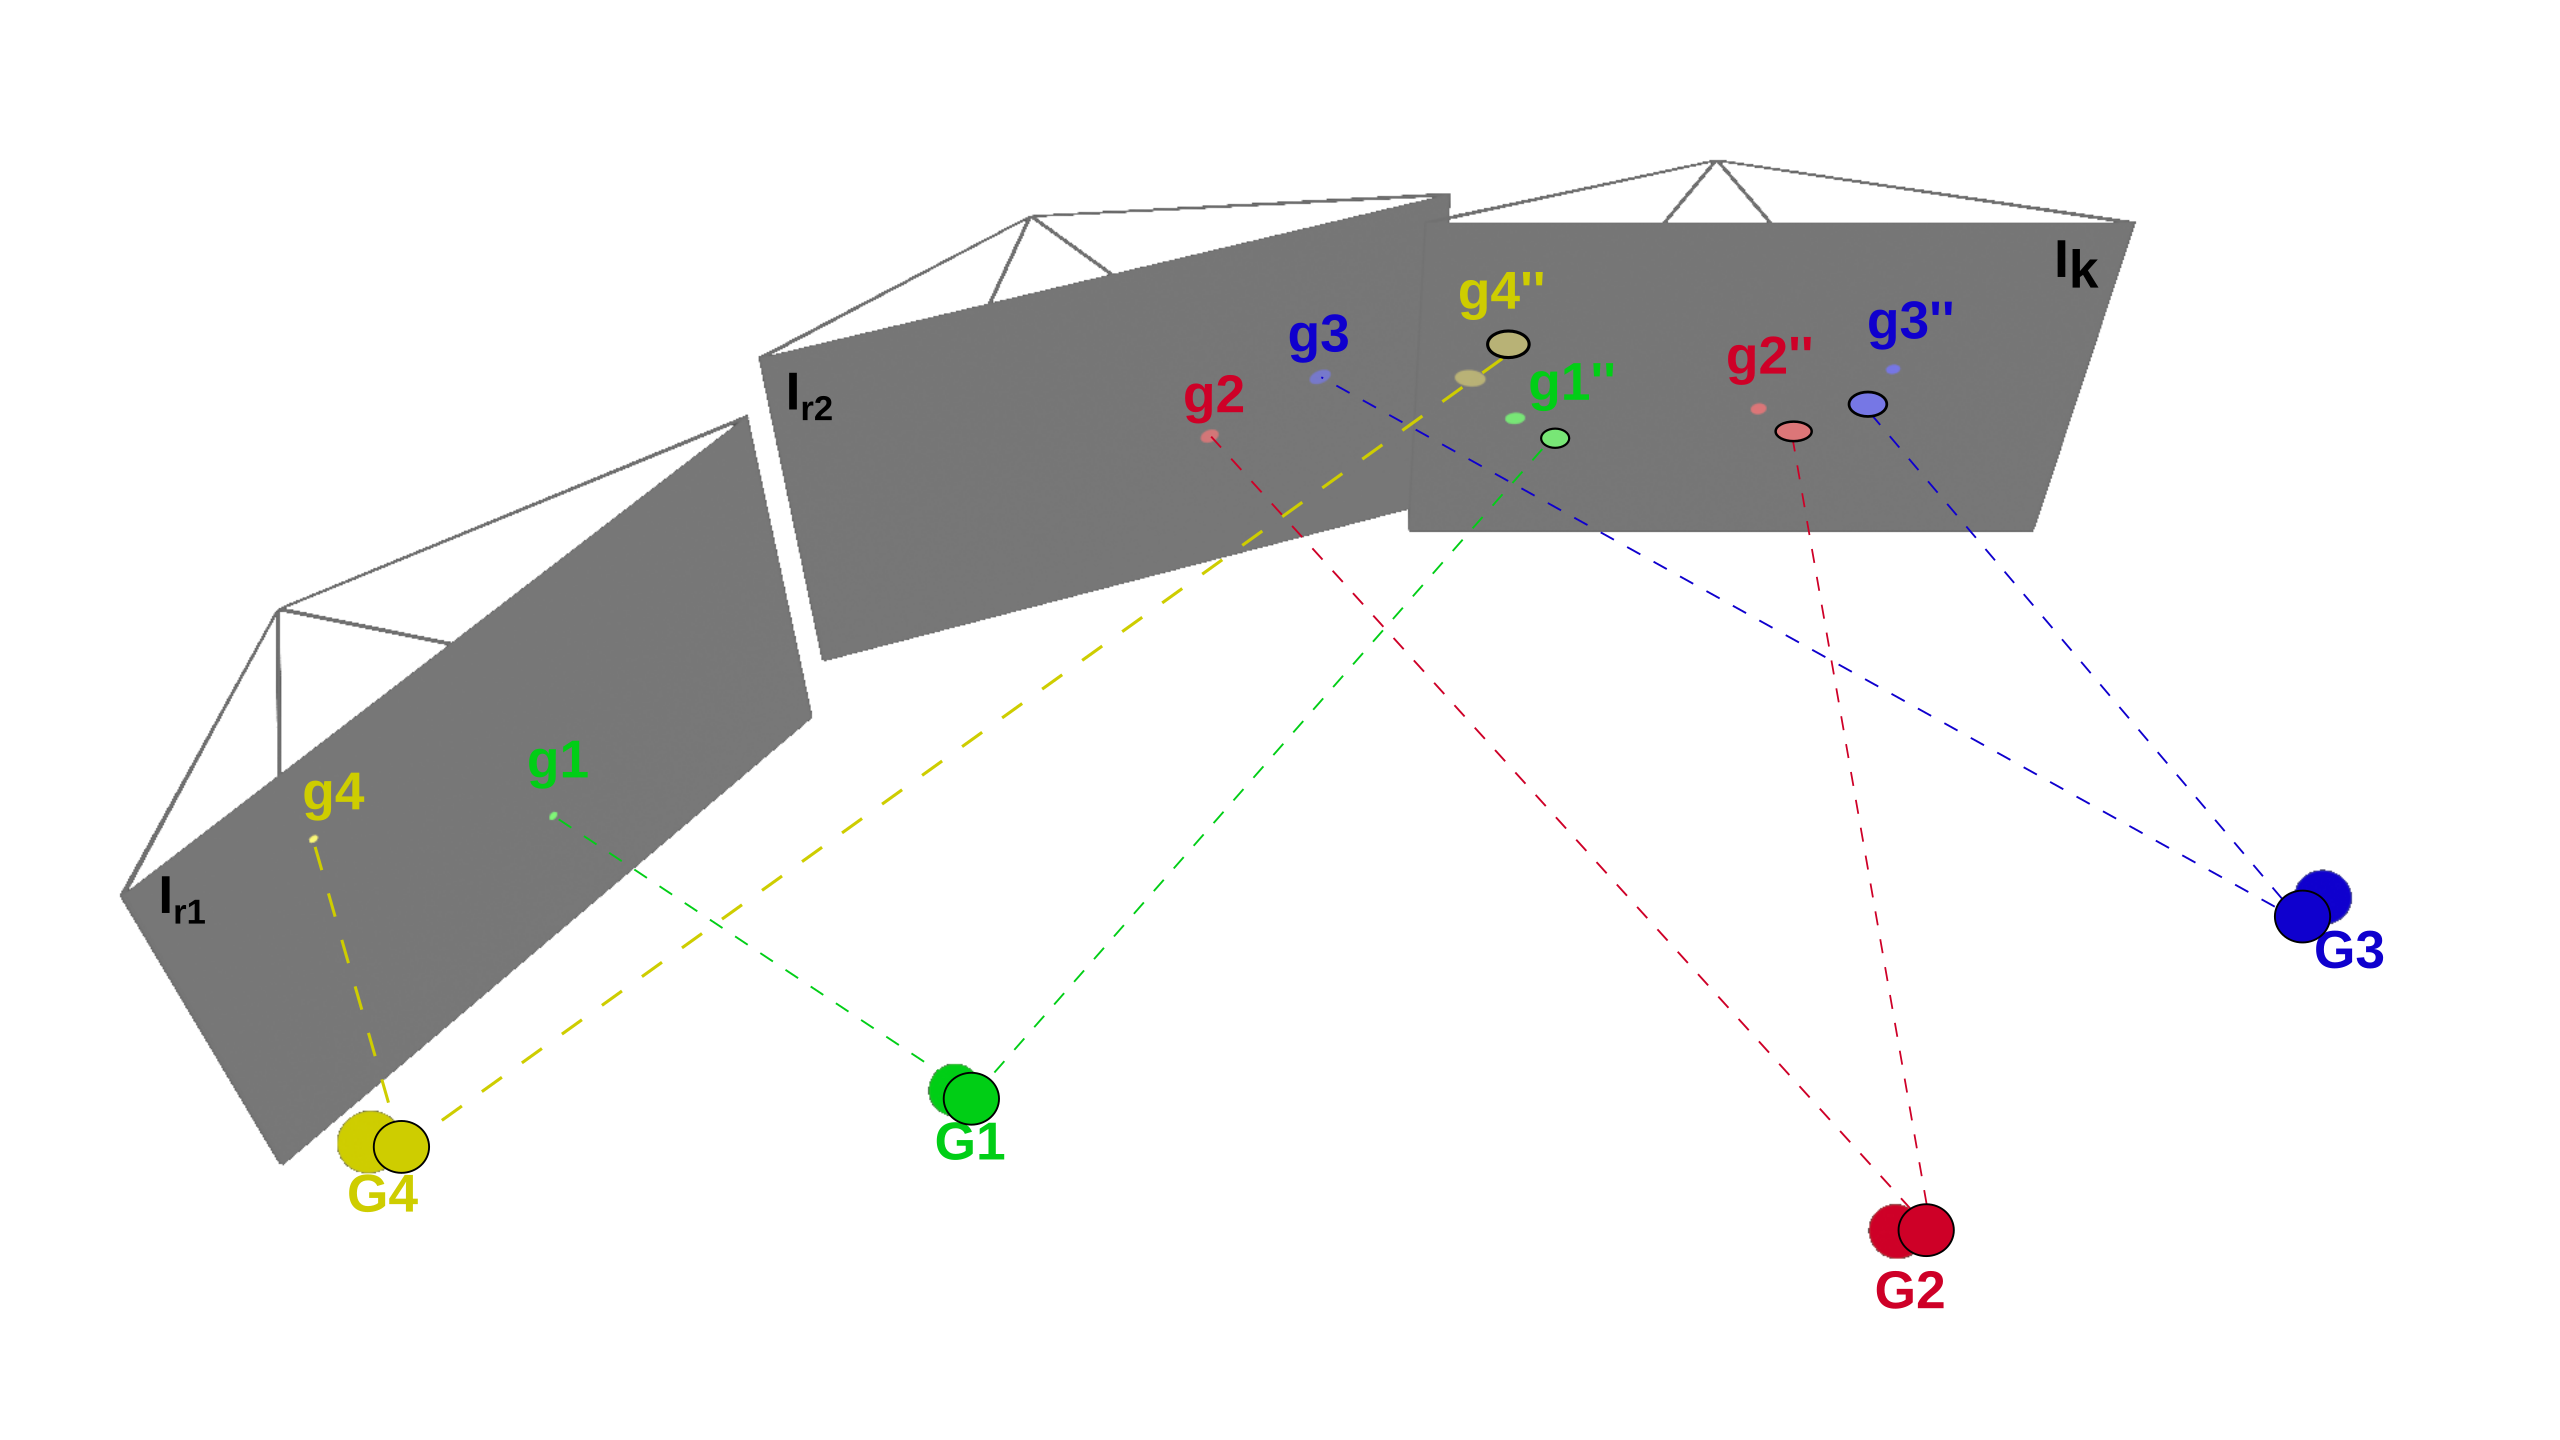
\includegraphics[height=0.9\textheight]{../img/pose_estimation_point_update.png}
  \end{center}
\end{frame}

\begin{frame}{Optical Flow}
  \begin{center}
    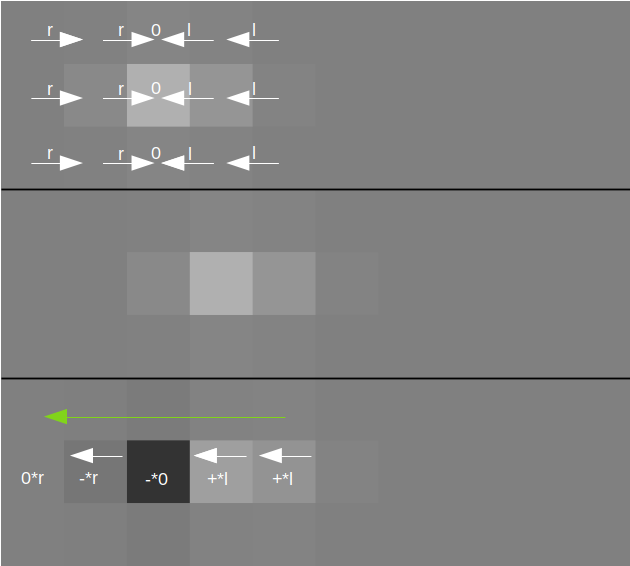
\includegraphics[height=0.9\textheight]{../img/optical_flow_intuitive_1.png}
  \end{center}
\end{frame}

\begin{frame}{Optical Flow}
  \begin{center}
    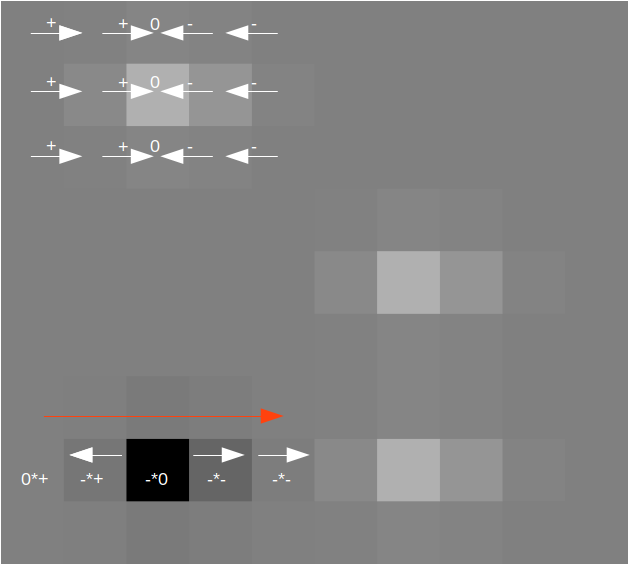
\includegraphics[height=0.9\textheight]{../img/optical_flow_intuitive_2.png}
  \end{center}
\end{frame}

\begin{frame}{Optical Flow}
  \begin{center}
    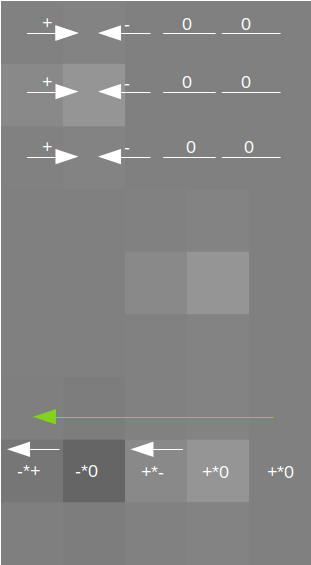
\includegraphics[height=0.9\textheight]{../img/optical_flow_intuitive_3.png}
  \end{center}
\end{frame}

\begin{frame}{Results (Blender Scene)}
  \begin{center}
    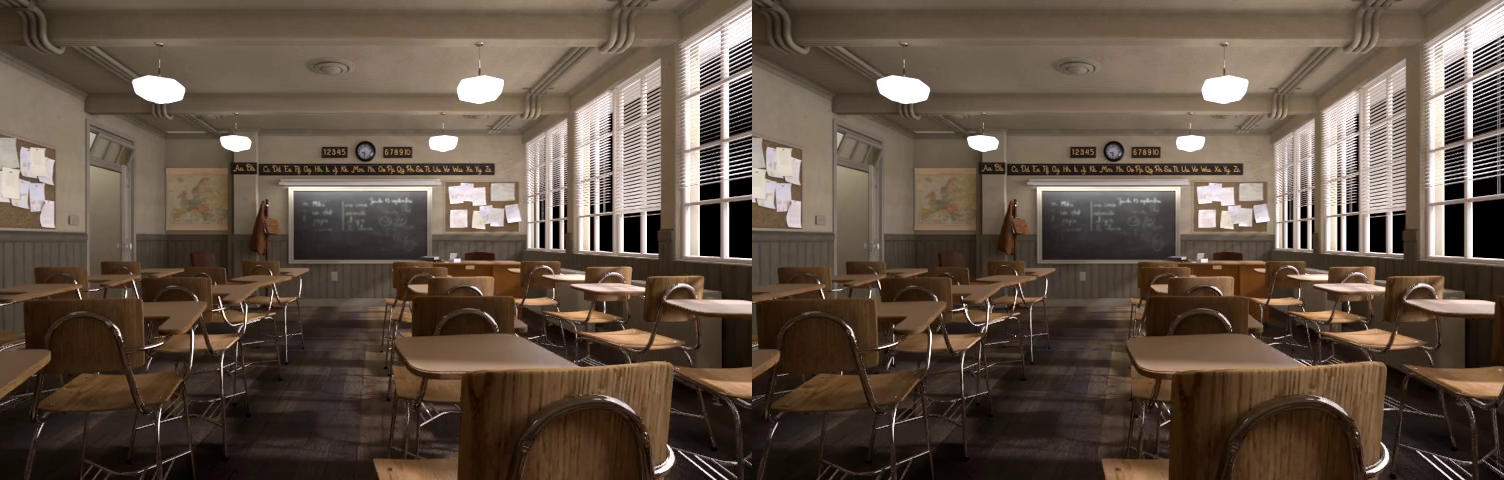
\includegraphics[width=0.9\textwidth]{../img/blender_classroom_scene.png}
  \end{center}
\end{frame}

\begin{frame}{Results}
  \begin{center}
    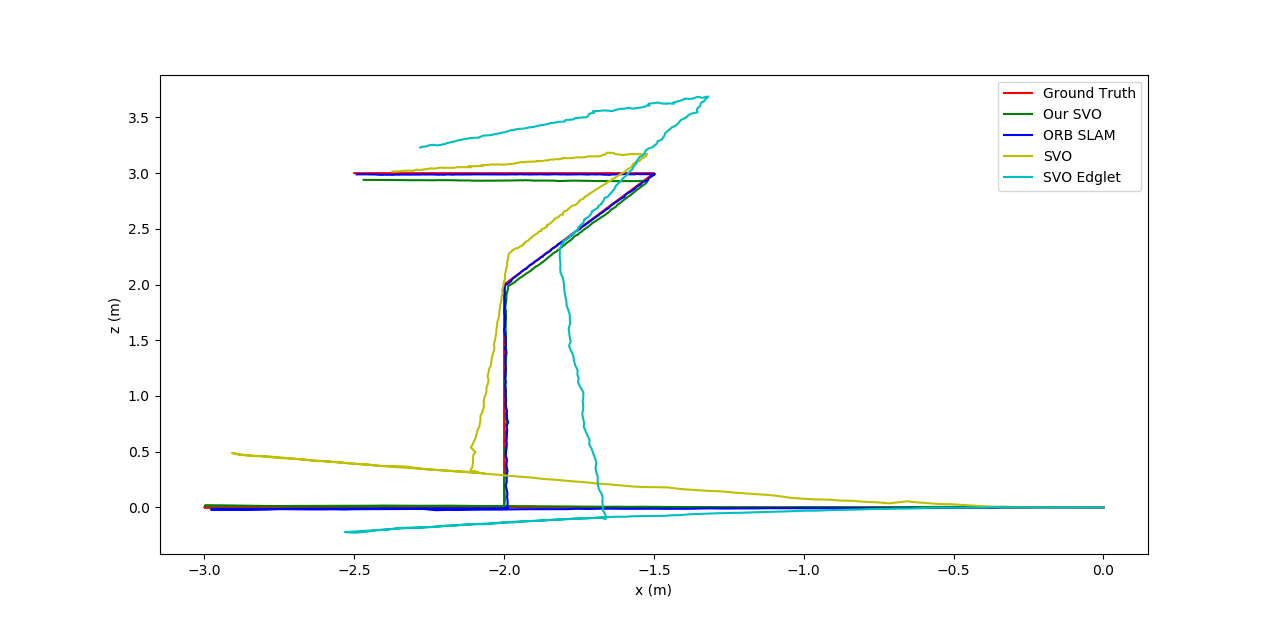
\includegraphics[height=0.9\textheight]{../img/blender_classroom_simple_comp_top.png}
  \end{center}
\end{frame}

\begin{frame}{Conclusion}
  \begin{columns}[c]
    \begin{column}{0.4\linewidth}
      \begin{itemize}
        \item Faster than ORB SLAM
        \item Not as accurate
        \item Good for embedded devices
        \item Less beneficial for CPVR lab
      \end{itemize}
    \end{column}
    \begin{column}{0.4\linewidth}
      \begin{center}
        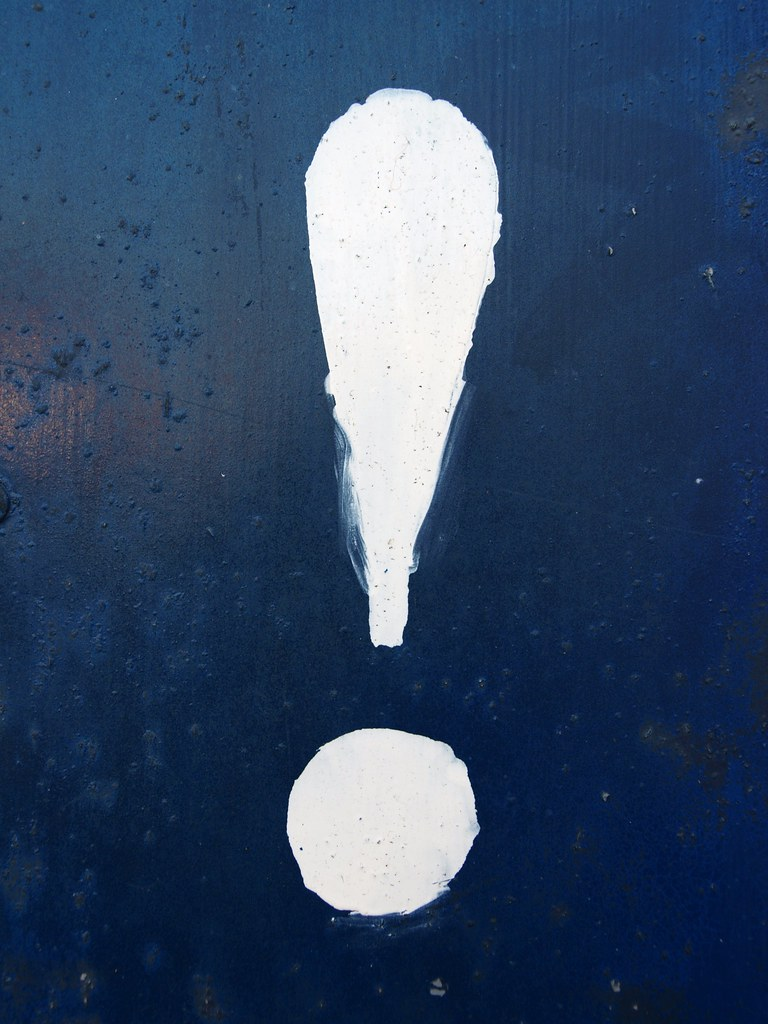
\includegraphics[width=0.5\textwidth]{./img/exclamationmark.jpg}
      \end{center}
    \end{column}
  \end{columns}
\end{frame}

\begin{frame}{Questions}
  \begin{center}
    
\includegraphics[height=0.9\textheight]{./img/question.jpg}
  \end{center}
  https://github.com/eichenberger/stereo-svo-slam
\end{frame}


\end{document}

